\section{Introduction}
For digitization projects, the construction industry is a mostly unconquered field yet.
On the one hand, the dynamic, sometimes harsh (e.g. weather influence, no infrastructure, etc.) environments of the construction site challenges the technology and adds harder requirements compared to an industrial application on the shop floor. 
On the other hand, the typically conservative and hierarchical work culture makes the introduction and acceptance of new methods more challenging. 
In this paper, we describe the vision and ideas behind the ConWearDi project and its approach to better understand and overcome these challenges.

\section{Project scope}
Construction projects vary in size and complexity highly (e.g. from huge civil engineering projects to building a small house). 
The project ConWearDi focuses its efforts on improving efficiency of smaller constructions, e.g. interior work and painting of houses, and craftsman businesses.
Challenges for these business are different, than those of a big multinational corporation with thousands of workers, but nonetheless very interesting and important.

\section{Problem description}
The construction industry shows a huge potential for digitization and it's still in the early phase of adopting technologies related to Industry 4.0. 
Meanwhile the Building Information Modeling (BIM) supports the processes of the design and planning phase, the actual construction, the execution process of the value creation, is still dominated by analog processes and paper documents. 
Examples include wall sized printed plans and time sheets on paper, which are only digitally recorded in the office and are available only there. 
So, in many cases, the digital world ends in the back office or at the workstations of the architects, managers and foremen. 
The potential of novel services, such as Internet of Things (IoT) systems with sensors and actuators deployed on site connecting it to powerful computing resources, remained untapped.

\section{Project goal}
Our goal in the ConWearDi project is the design and prototype implementation of a platform capable to capture and analyze the current state of the construction work and to provide useful informational support not only for the managers and architects but directly to the construction workers and craftsmen on site. 

%Information sources, which provide structured information and accurate specifications (e.g. used materials) about a project, such as the BIM itself, are the foundation to achieve this goal. These

The main project goals can be summarized as:
\begin{enumerate}
  \item Creation of a Digital Twin, a representation of the construction site, which always reflects its current state 
  \item Centralized system for managing the construction site
  \item Automatic documentation for knowledge- and quality management purposes
  \item Exploration of new business models
  \item Development of methods for monitoring the activities of different worker groups with wearable technologies
\end{enumerate}

\section{Vision}

\begin{figure*}[htp]
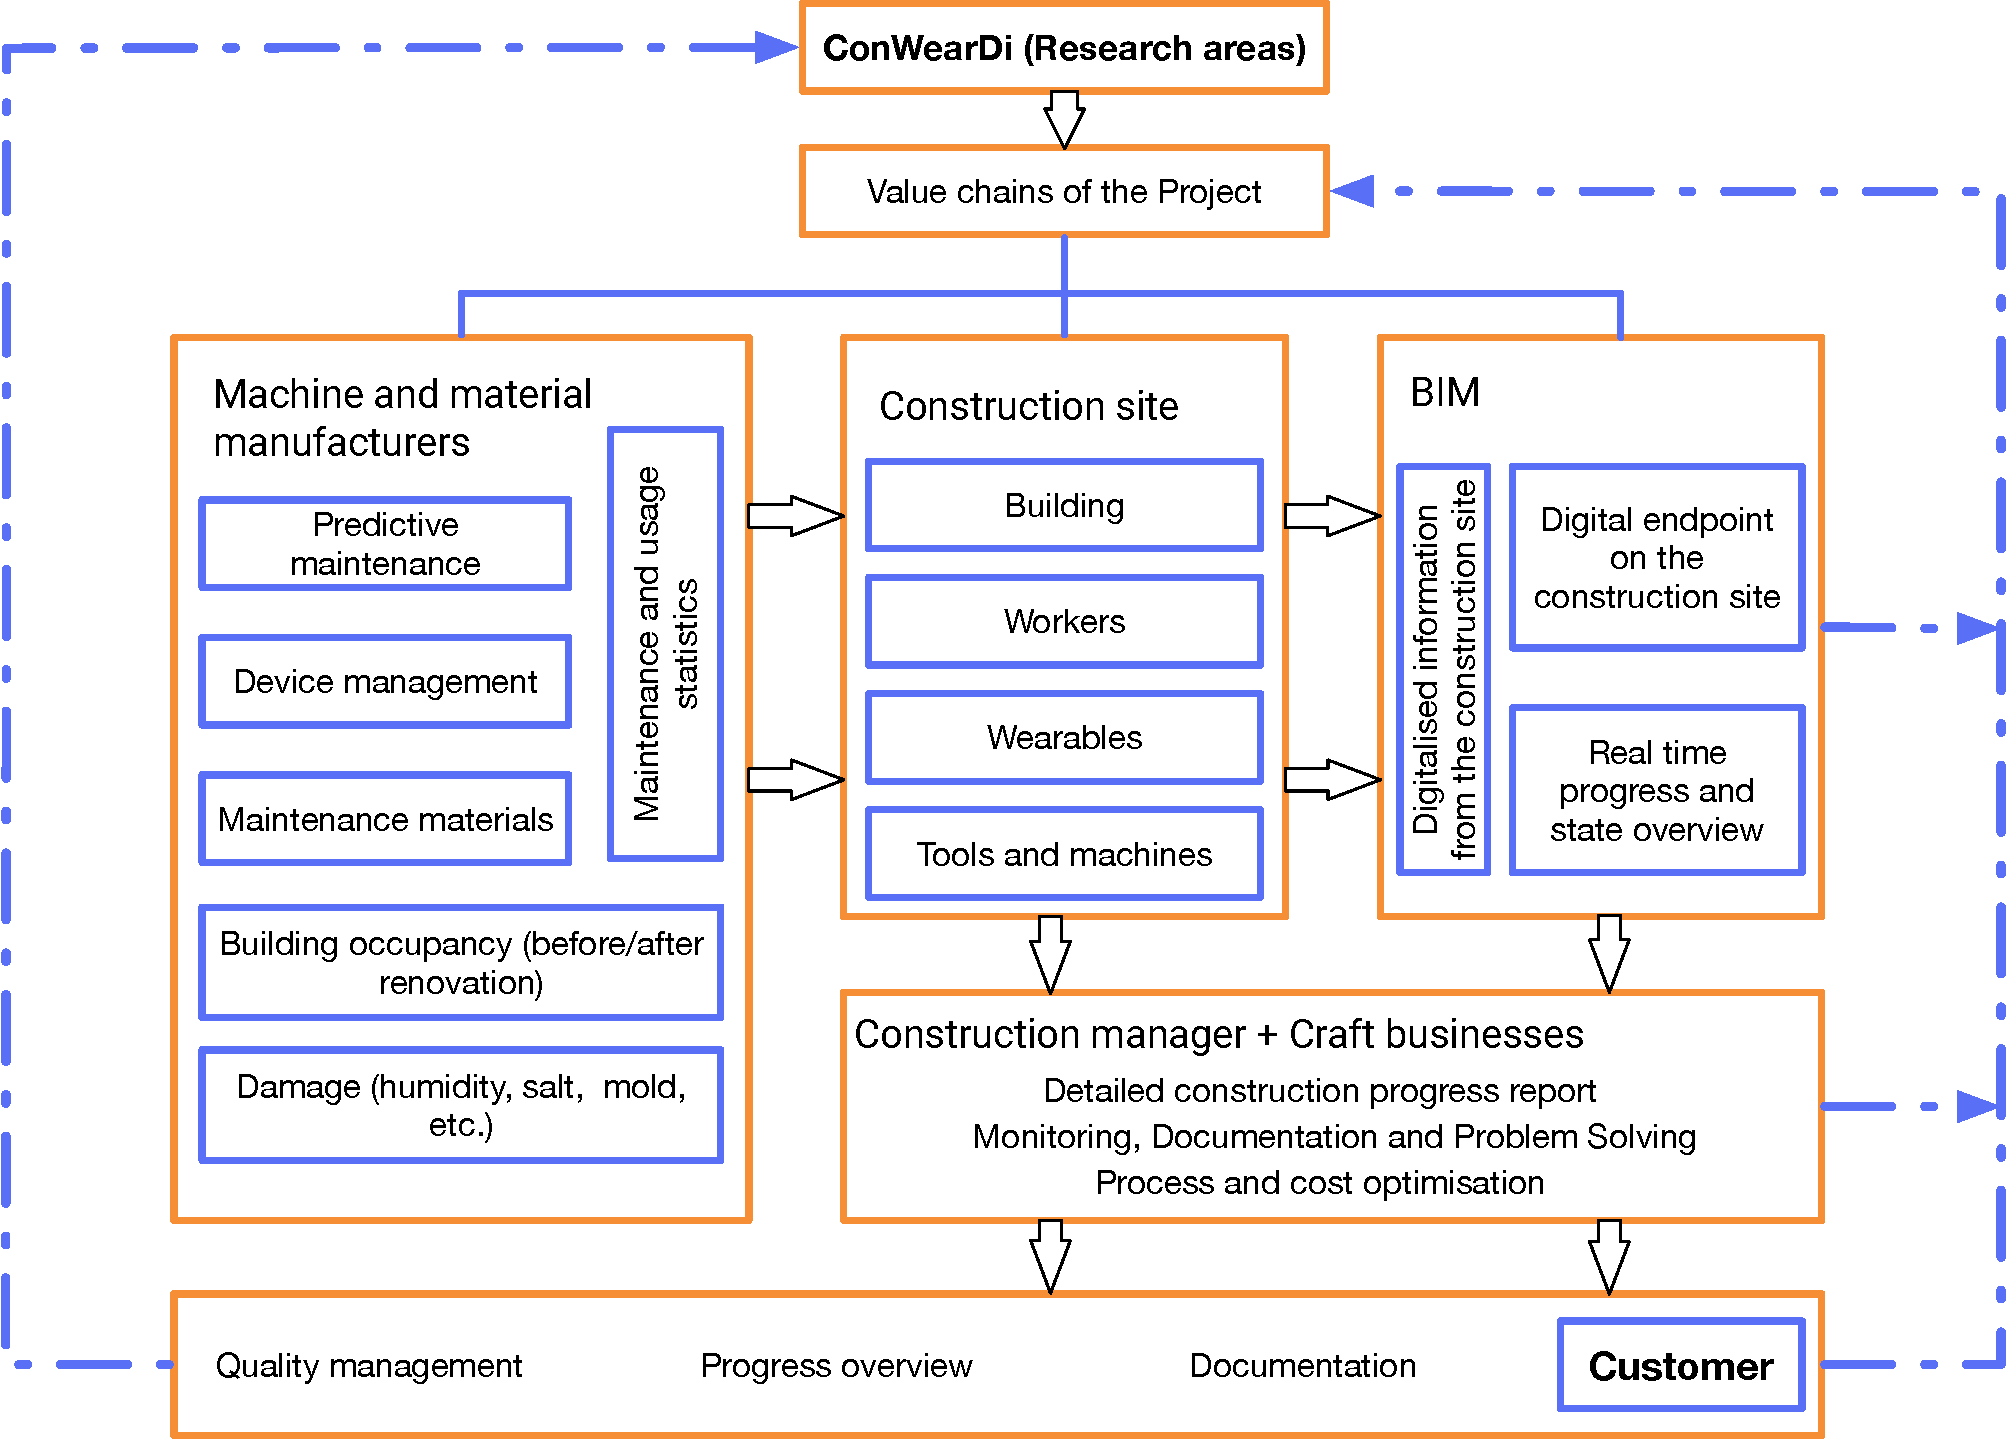
\includegraphics[width=0.8\textwidth]{figures/conweardi-functional}
\caption{Functional graph}
\label{fig:functional}
\end{figure*}

The most significant benefit, we envision through realization of the ConWearDi system, is better efficiency in detecting and preventing problems and damages by improving or if possible automatizing construction site documentation and reporting workflows.
With the real time information flow from the construction site, planners and managers are able to anticipate upcoming issues and avoid costly delays and damage repairs.
Communication between customers, managers, designers and workers will also be improved by bundling of information such as agreements, used materials, tools and recorded working hours. 

\todo{translate}
Die folgenden Dienstleistungen mit Bezug zur Bauausführung sollen durch ConWearDi ermöglicht oder signifikant verbessert werden. Dadurch werden signifikante, messbare Verbesserungen im „magischen“ Zieldreieck Termineinhaltung, Kosten und Qualität erzielt und somit der  Kundennutzen und die Kundenzufriedenheit, aber auch die Produktivität und Wirtschaftlichkeit der am Bau beteiligten Unternehmen, deren Mitarbeiternutzen und die Arbeitszufriedenheit (“die richtigen Informationen zur richtigen Zeit am richtigen Ort) sowie die Wirtschaftlichkeit und der Nutzen von Maschinen und Materialherstellern deutlich erhöht.

Für den Bauleiter:
- Rückmeldewesen ähnlich der Industrieproduktion, IST-Stand der Baustelle ständig live verfügbar, Baufortschritt fortlaufend und Störungen vorhersehbar für alle Beteiligten erkennbar
- Detaillierte Baufortschrittsdokumentation, "Die Sanierung des Gebäudes dokumentiert ihre Entstehung"
- Detaillierte Lösungsdokumentation, „Das Gebäude dokumentiert seine innere Struktur, insbesondere verborgene Teile“
- Notwendigkeit für Lösungsfindung sofort erkennbar, Schnittstellenprobleme frühzeitig erkennbar und jederzeit transparent
- kooperative Lösungsfindung, um die  Planung zu  konkretisieren  oder  modifizieren 
- laufend detaillierte Überwachung von Zeiten, Kosten und Kalkulationsansätzen (Zeit und Materialverbrauch), Fortschritt und Ressourcenauslastung
- Sicherstellung der Unterweisung und Einhaltung der Vorgaben zu Arbeitssicherheit und Gesundheitsschutz
- Lernen aus durchgeführten Projekten (Grundlage für Prädiktion) 


Für den Planer und Projektsteuerer:
- digital dokumentierte Commitments, statt mündlicher Absprachen
- vereinfachte, IT-gestützte Gewerke-Koordination auf Basis von Advanced Planning and Scheduling (APS)
- Unterstützung zukünftiger Standards der Dokumentation, z.B. im Brandschutz
- BigData Analytics Dienste auf hohem Daten-Detailgrad und über Bauprojekte hinweg


Für Hersteller und Lieferanten von Maschinen, Werkzeugen und Materialien:
- Effiziente Einsatz- und Logistikkoordinierung 
- proaktive Service- und Wartungsplanung für Baumaschinen durch Auslastungs- und Abnutzungstracking.
- Proaktive Instandhaltung von eingebauten Materialien durch Tracking von Zustand und bauphysikalischen Daten (z.B. Feuchte, Temperatur) 
- Fortwährende Erkenntnisse über Verbesserungs- und Optimierungspotenzial auf der Grundlage kontinuierlicher Sensordaten


Für den Handwerksunternehmer und Handwerker auf der Baustelle
- kontextbezogene, rückfragefreie Informationen zur Sicherung der Ausführungsqualität und Arbeitssicherheit
- Echtzeit-Remote-Supportmöglichkeiten zu allen Beteiligten (Planer, Maschinen- und Materialhersteller, Unternehmer)
- Meldewesen für Störungen und Integration jedes Einzelnen in den kontinuierlichen Verbesserungsprozess, dadurch Erhöhung der Arbeitszufriedenheit
- Echtzeit-Produktivitätsmessung, Soll-/Ist-Abgleich prozessorientierter Arbeitsablaufpakete mit der Möglichkeit zur Simulation von Alternativen
- optimierter Ressourceneinsatz und Entscheidungsunterstützung durch intelligentes, variantenfähiges Scheduling anhand von digitalen Echtzeitdaten von der Baustelle


\section{Methodology}
\todo{to succeed with the complex task - include experts from different professions and stakeholders}
\todo{figure describes the main functional process of the project - ... describe here }
Figure \ref{fig:functional}

\todo{project partners, who is doing what}

\todo{add paper references here to previous works of the groups}

Die Prozessverschiebung digitaler Endpunkte erfolgt in die wertschöpfenden Tätigkeiten auf der Baustelle, der eigentlichen Bautätigkeit. Zu diesem Zweck werden im Projekt ein Baugerätehersteller (Firma Wagner, Spritzmaschinen), ein Materialhersteller (DAW), ein mittelständischer Hersteller von ERP Software für Bauunternehmen (Sander + Partner GmbH), mehrere Handwerks-/Baubetriebe sowie Forschungsgruppen aus den Bereichen Internet of Things (DFKI), Prozessplanung (ITWM + eBZ) und Psychologie (TU KL) zusammenarbeiten. Seitens der Technologie werden die Baumitarbeiter mit Wearables (tragbare Computersysteme) ausgestattet und auf der Baustelle kommen intelligente Maschinen (konkret z.B. Spritzmaschinen für Malerarbeiten), sowie in Materialien integrierte Sensoren zum Einsatz (z.B. Sensoren in der Wärmedämmung).

Dabei sollen Lösungen erarbeitet werden die es (1.) Geräteherstellern erlauben eine proaktive Wartung der Geräte auf der Baustelle vorzunehmen, (2.) Materialherstellern eine proaktive Instandhaltung der verbauten Materialien, (3.) neue Geschäftsmodelle ermöglicht (z.B. “just in time”-Geräteleasing, kundenbezogen Marketingmethode), und (4.) eine datengetriebene Weiterentwicklung der Produkte und Dienstleistungen durch von vielen Kunden gesammelte „BigData“ erlauben. Des Weiteren sollen reale Bauprozesse durch digitale Echtzeitinformation ihrer Repräsentation in den ERP-Systemen synchronisiert werden. So können Bauprozesse im Sinne von Effizienz, Qualitätssicherung und Arbeitssicherheit überwacht und gesteuert werden. Dadurch kann auch dem Baukunden ein einmaliger vertrauensbildender Zugang und eine einmalige Dokumentation zum Bauprozess als Dienstleistung geboten werden.
Die aufgeführten Projektergebnisse sind in der nachfolgenden Funktionsgrafik in ihrer Wirkungsbeziehung dargestellt.


\section{Conclusion}
\todo{high potential to digization - still many unsolved problems - project is focusing to making first demonstrators - running at first real businesses}

\todo{for more information visit project website}

\begin{acks}
  \todo{BMBF founded project}
  
  The work is
  supported by the \grantsponsor{GS501100001809}{National Natural
    Science Foundation of
    China}{http://dx.doi.org/10.13039/501100001809} under Grant
  No.:~\grantnum{GS501100001809}{61273304}
  and~\grantnum[http://www.nnsf.cn/youngscientists]{GS501100001809}{Young
    Scientists' Support Program}.

\end{acks}
